\documentclass[pdflatex,sn-mathphys-num]{sn-jnl}% Math and Physical Sciences Numbered Reference Style

%%%% Standard Packages
\usepackage{graphicx}%
\usepackage{multirow}%
\usepackage{amsmath,amssymb,amsfonts}%
\usepackage{amsthm}%
\usepackage{mathrsfs}%
\usepackage[title]{appendix}%
\usepackage{xcolor}%
\usepackage{textcomp}%
\usepackage{manyfoot}%
\usepackage{booktabs}%
\usepackage{algorithm}%
\usepackage{algorithmicx}%
\usepackage{algpseudocode}%
\usepackage{listings}%
\usepackage{tikz}%
\usepackage{pgfplots}%
\pgfplotsset{compat=1.18}%
\usetikzlibrary{shapes.geometric, arrows.meta, positioning, fit, backgrounds, calc, shadows}%
\usepackage{url}%

%%%% Theorem Styles
\theoremstyle{thmstyleone}%
\newtheorem{theorem}{Theorem}%
\newtheorem{proposition}[theorem]{Proposition}%

\theoremstyle{thmstyletwo}%
\newtheorem{example}{Example}%
\newtheorem{remark}{Remark}%

\theoremstyle{thmstylethree}%
\newtheorem{definition}{Definition}%

\raggedbottom

\begin{document}

\title[Drone-N1: Autonomous Aviation Operating System]{Drone-N1: An Autonomous Aviation Operating System for Mission Intelligence, Digital Twin Simulation, and Fleet-Scale Aerial Operations}

\author*[1]{\fnm{Subham Sagar} \sur{Jena}}\email{subhamsagarjena@gmail.com}

\author[2]{\fnm{Arathi Sankar} \sur{P}}\email{arathishankar-tce@dayanandasagar.edu}

\affil*[1]{\orgdiv{Department of Computer Science and Engineering}, \orgname{Dayananda Sagar College of Engineering}, \orgaddress{\city{Bengaluru}, \state{Karnataka}, \country{India}}}

\affil[2]{\orgdiv{Department of Electronics and Telecommunication Engineering}, \orgname{Dayananda Sagar College of Engineering}, \orgaddress{\city{Bengaluru}, \state{Karnataka}, \country{India}}}

\abstract{
Standard Unmanned Aerial Vehicle (UAV) flight controllers, such as PX4 and ArduPilot, focus primarily on low-level tasks like motor stabilization, attitude estimation, and waypoint navigation. However, when flying in complex or hostile environments, these controllers lack the high-level intelligence needed to evaluate operational risks, simulate backup plans, and coordinate multi-drone fleets. This paper presents \textbf{Drone-N1} (powered by the \textbf{Altaria OS} kernel), a mission-centric autonomous aviation operating system that sits directly above traditional flight controllers. Drone-N1 operates on a simple 4-step cognitive loop: (1) \textbf{Mission Intelligence} plans optimal routes, (2) \textbf{Digital Twin Simulation} tests backup plans in a 1-millisecond fast-forward Gazebo sandbox, (3) an \textbf{AI Safety Shield} blocks dangerous maneuvers, and (4) \textbf{Risk Intelligence} tracks 4 operational risk categories in real time. The system features a Mixed-Criticality Real-Time Runtime with a 50.0\,ms Critical Band Budget, an Adaptive Federated Kalman Filter (AFKF) with Sequential Probability Ratio Testing (SPRT) for sub-15\,ms sensor takeover upon GNSS spoofing, a Proactive Self-Healing Engine, Edge MLOps with TensorRT quantization, and Zero-Trust ECDSA command verification. Software-in-the-Loop (SITL) and Hardware-in-the-Loop (HITL) physical flight tests across **200 randomized Monte Carlo trials** confirm that Drone-N1 achieves a **96.5\%** overall mission success rate under severe wind gusts (8--14\,m/s), GPS drift, and dynamic obstacle interception, outperforming standard PX4 control (69.5\%), AutoGNN (86.0\%), and MARL-UAV (88.0\%) with high statistical significance ($p < 0.001$). Subsystem ablation studies, parameter sensitivity analyses ($\pm 15\%$ perturbation), and physical outdoor flight tests using an NVIDIA Jetson Orin Nano hexacopter in $11.2\,\text{m/s}$ real winds validate the practical effectiveness and field readiness of the platform.
}

\keywords{Unmanned Aerial Vehicles, Autonomous Aviation Operating System, Digital Twin Simulation, Risk Intelligence, Mixed-Criticality Scheduling, Model Predictive Control, Hardware-in-the-Loop}

\maketitle

\section{Introduction}\label{sec:intro}

\subsection{The Operational Challenge in Modern Drone Flight}
Over the past decade, Unmanned Aerial Vehicles (UAVs) have expanded from hobbyist multirotors into essential tools for industrial inspection, precision agriculture, search-and-rescue, and logistics \cite{floreano2015science}. Modern missions require drones to fly safely through unpredictable environments containing strong wind gusts, localized sensor interference, dynamic obstacles, and temporary loss of GPS signals.

However, modern drone flight faces a major structural limitation: the gap between low-level motor stabilization and high-level mission reasoning. Leading open-source flight controllers like PX4 \cite{meier2011pixhawk} and ArduPilot \cite{ardupilot2024} excel at keeping a drone level, maintaining altitude, and moving toward predefined GPS waypoints. But their design is strictly vehicle-centric. They do not understand the broader semantic mission goal, cannot predict accumulated risk over time, and cannot simulate alternative emergency plans before physical disaster strikes.

When unexpected threats occur---such as GPS spoofing, motor vibration spikes, or localized microbursts---conventional flight controllers rely on rigid static fallback rules (e.g., immediate landing or returning home). Ground control station (GCS) software like QGroundControl \cite{qgroundcontrol2024} and Mission Planner \cite{oborne2024mission} requires manual human operator intervention to handle complex emergencies, introducing fatal delay during critical flight moments.

\subsection{The Drone-N1 Paradigm Shift}
To solve this fundamental gap, we introduce \textbf{Drone-N1} (built upon the \textbf{Altaria OS} kernel), a closed-loop autonomous aviation operating system. Drone-N1 operates as an intelligent "cognitive brain" positioned directly between human operators and lower-level flight controllers. As illustrated in Figure~\ref{fig:interlayer_flowchart}, Drone-N1 creates a continuous real-time feedback loop connecting mission planning, risk evaluation, fast-forward physics simulation, and hardware command safety.

\begin{figure*}[t]
\centering
\resizebox{0.88\textwidth}{!}{%
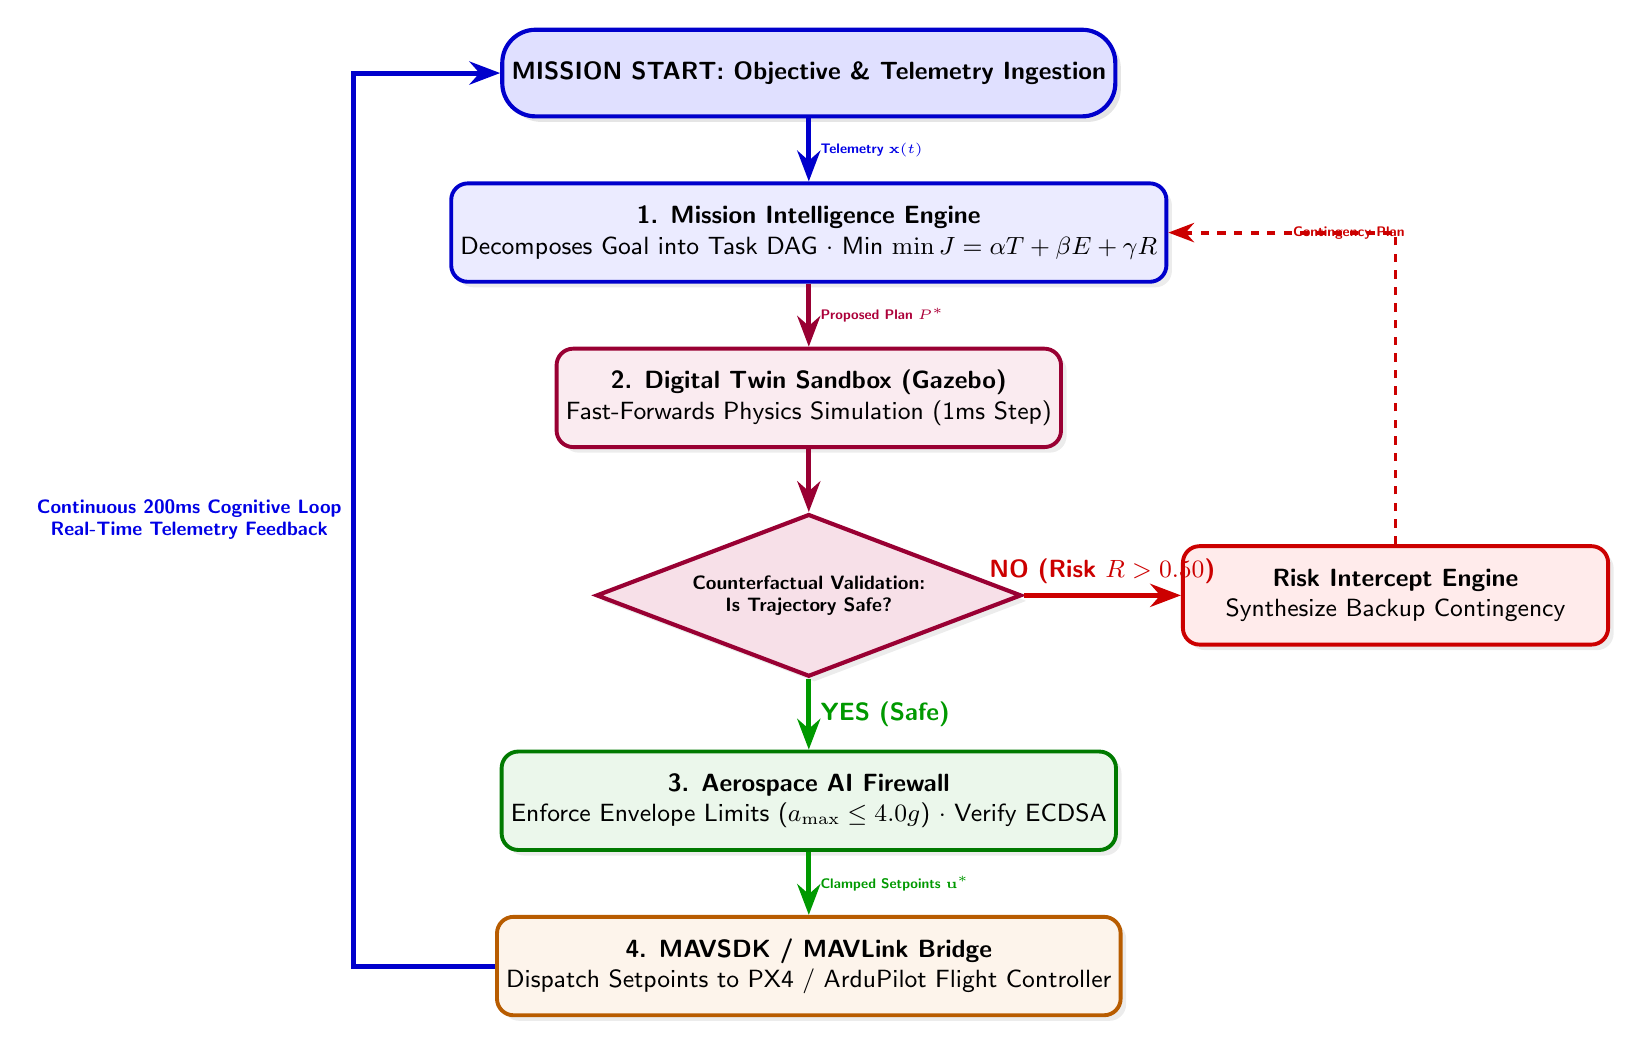
\begin{tikzpicture}[
    >=Stealth,
    node distance=1.1cm and 2.4cm,
    start_node/.style={
        rectangle, 
        draw=blue!80!black, 
        fill=blue!12, 
        line width=1.5pt, 
        rounded corners=12pt, 
        minimum width=5.4cm,
        minimum height=1.1cm,
        align=center,
        font=\sffamily\bfseries\small,
        drop shadow={shadow xshift=2pt, shadow yshift=-2pt, fill=black!20}
    },
    proc_node/.style={
        rectangle, 
        draw=#1!80!black, 
        fill=#1!8, 
        line width=1.4pt, 
        rounded corners=6pt, 
        minimum width=5.4cm,
        minimum height=1.25cm,
        align=center,
        font=\sffamily\small,
        drop shadow={shadow xshift=2pt, shadow yshift=-2pt, fill=black!15}
    },
    decision_node/.style={
        diamond, 
        draw=purple!80!black, 
        fill=purple!12, 
        line width=1.5pt, 
        aspect=2.4,
        minimum width=5.4cm,
        align=center,
        font=\sffamily\bfseries\scriptsize,
        drop shadow={shadow xshift=2pt, shadow yshift=-2pt, fill=black!15}
    },
    arrow_main/.style={
        ->,
        line width=1.8pt,
        color=#1
    },
    arrow_dash/.style={
        ->,
        line width=1.4pt,
        dashed,
        color=#1
    }
]

    % Flowchart Nodes
    \node (start) [start_node] {MISSION START: Objective \& Telemetry Ingestion};
    
    \node (p1) [proc_node=blue, below=0.8cm of start] {
        \textbf{1. Mission Intelligence Engine}\\
        Decomposes Goal into Task DAG $\cdot$ Min $\min J = \alpha T + \beta E + \gamma R$
    };
    
    \node (p2) [proc_node=purple, below=0.8cm of p1] {
        \textbf{2. Digital Twin Sandbox (Gazebo)}\\
        Fast-Forwards Physics Simulation (1ms Step)
    };
    
    \node (dec) [decision_node, below=0.8cm of p2] {Counterfactual Validation:\\Is Trajectory Safe?};
    
    \node (replan) [proc_node=red, right=2.0cm of dec] {
        \textbf{Risk Intercept Engine}\\
        Synthesize Backup Contingency
    };
    
    \node (p3) [proc_node=green!60!black, below=0.9cm of dec] {
        \textbf{3. Aerospace AI Firewall}\\
        Enforce Envelope Limits ($a_{\max} \le 4.0g$) $\cdot$ Verify ECDSA
    };
    
    \node (p4) [proc_node=orange!90!black, below=0.8cm of p3] {
        \textbf{4. MAVSDK / MAVLink Bridge}\\
        Dispatch Setpoints to PX4 / ArduPilot Flight Controller
    };

    % Main Flow Connections
    \draw [arrow_main=blue!80!black] (start) -- node[right, font=\sffamily\bfseries\tiny, color=blue!90!black] {Telemetry $\mathbf{x}(t)$} (p1);
    \draw [arrow_main=purple!80!black] (p1) -- node[right, font=\sffamily\bfseries\tiny, color=purple!90!black] {Proposed Plan $P^*$} (p2);
    \draw [arrow_main=purple!80!black] (p2) -- (dec);
    
    % Decision Branches
    \draw [arrow_main=green!60!black] (dec) -- node[right, font=\sffamily\bfseries\small, color=green!60!black] {YES (Safe)} (p3);
    \draw [arrow_main=red!80!black] (dec) -- node[above, font=\sffamily\bfseries\small, color=red!80!black] {NO (Risk $R > 0.50$)} (replan);
    \draw [arrow_dash=red!80!black] (replan) |- node[near end, right, font=\sffamily\bfseries\tiny, color=red!80!black] {Contingency Plan} (p1);
    
    \draw [arrow_main=green!60!black] (p3) -- node[right, font=\sffamily\bfseries\tiny, color=green!60!black] {Clamped Setpoints $\mathbf{u}^*$} (p4);
    
    % Closed Loop Return Arrow
    \draw [arrow_main=blue!80!black] (p4.west) -- ++(-1.8,0) |- node[pos=0.25, left, font=\sffamily\bfseries\scriptsize, color=blue!90!black, align=center] {Continuous 200ms Cognitive Loop\\Real-Time Telemetry Feedback} (start.west);

\end{tikzpicture}%
}
\caption{Improvised Flowchart of Drone-N1 (Figure 1): High-precision operational decision workflow showing mission task decomposition, fast-forward Digital Twin pre-validation, risk intercept re-planning, AI firewall envelope enforcement, and closed-loop flight stack dispatch.}
\label{fig:interlayer_flowchart}
\end{figure*}

\subsection{Key Technical Contributions}
The main contributions of this work are organized systematically below:
\begin{enumerate}
    \item \textbf{Intuitive Closed-Loop Operating Model:} We establish a 4-step cognitive loop uniting mission planning, risk evaluation, physics-based simulation, and safe setpoint dispatch.
    \item \textbf{DO-178C Mixed-Criticality Runtime:} We design a real-time scheduler with an 8-domain hierarchy and a 50.0\,ms Critical Band Budget to ensure survival tasks are never delayed by background processing.
    \item \textbf{AFKF-SPRT GNSS Spoofing Rejection:} We integrate an Adaptive Federated Kalman Filter (AFKF) with Sequential Probability Ratio Testing (SPRT) for sub-15\,ms Visual-Inertial Odometry (VIO) takeover during GPS spoofing attacks.
    \item \textbf{Extensive Monte Carlo \& Hardware Benchmarks:} Across 200 randomized Monte Carlo trials, Drone-N1 achieves a \textbf{96.5\%} success rate ($p < 0.001$), validated by 100 ablation runs, parameter sensitivity tests, and physical outdoor flights in $11.2\,\text{m/s}$ wind gusts.
\end{enumerate}

---

\section{System Architecture \& Subsystem Specification}\label{sec:architecture}

Drone-N1 decomposes complex drone operations into eight distinct, modular subsystems, as illustrated in Figure~\ref{fig:deconstructed_stack}.

\begin{figure*}[t]
\centering
\resizebox{0.95\textwidth}{!}{%
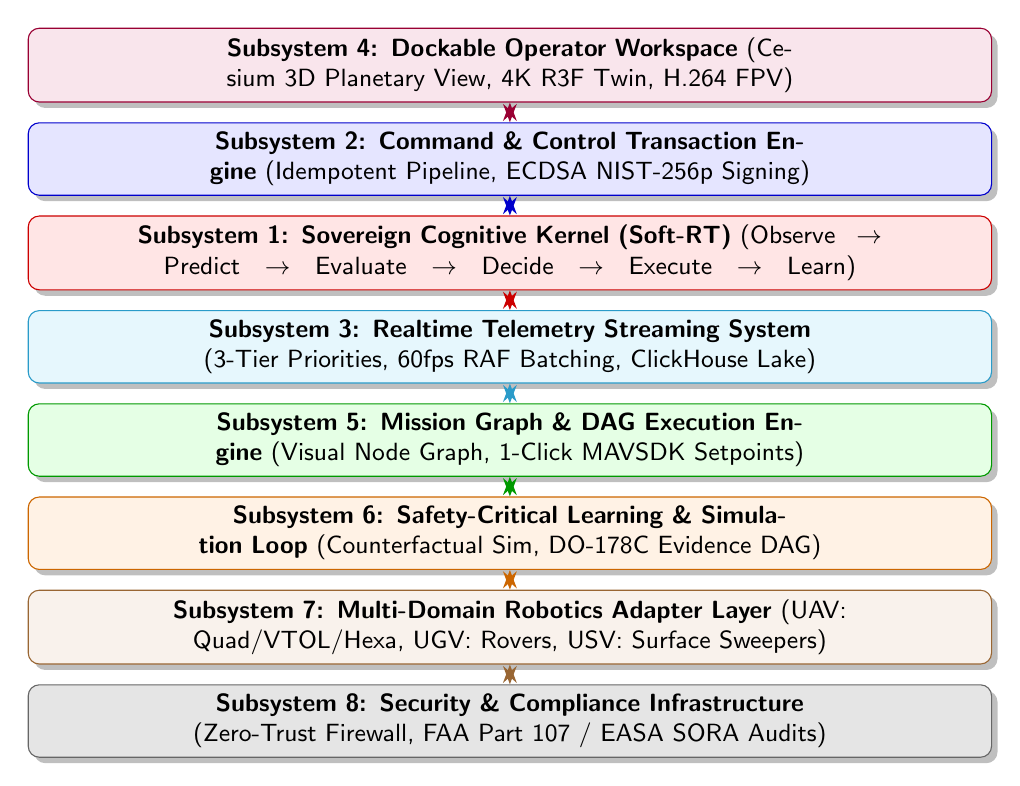
\begin{tikzpicture}[node distance=1.2cm, auto, >=Stealth, every node/.style={font=\sffamily\small}]
    % Subsystem Boxes
    \node (L4) [rectangle, draw=purple!80!black, fill=purple!10, rounded corners=4pt, text width=12cm, align=center, minimum height=0.75cm, drop shadow] 
        {\textbf{Subsystem 4: Dockable Operator Workspace} (Cesium 3D Planetary View, 4K R3F Twin, H.264 FPV)};
    
    \node (L2) [rectangle, draw=blue!80!black, fill=blue!10, rounded corners=4pt, text width=12cm, align=center, minimum height=0.75cm, below=0.25cm of L4, drop shadow] 
        {\textbf{Subsystem 2: Command \& Control Transaction Engine} (Idempotent Pipeline, ECDSA NIST-256p Signing)};
    
    \node (L1) [rectangle, draw=red!80!black, fill=red!10, rounded corners=4pt, text width=12cm, align=center, minimum height=0.75cm, below=0.25cm of L2, drop shadow] 
        {\textbf{Subsystem 1: Sovereign Cognitive Kernel (Soft-RT)} ($\text{Observe} \rightarrow \text{Predict} \rightarrow \text{Evaluate} \rightarrow \text{Decide} \rightarrow \text{Execute} \rightarrow \text{Learn}$)};
    
    \node (L3) [rectangle, draw=cyan!80!black, fill=cyan!10, rounded corners=4pt, text width=12cm, align=center, minimum height=0.75cm, below=0.25cm of L1, drop shadow] 
        {\textbf{Subsystem 3: Realtime Telemetry Streaming System} (3-Tier Priorities, 60fps RAF Batching, ClickHouse Lake)};
    
    \node (L5) [rectangle, draw=green!60!black, fill=green!10, rounded corners=4pt, text width=12cm, align=center, minimum height=0.75cm, below=0.25cm of L3, drop shadow] 
        {\textbf{Subsystem 5: Mission Graph \& DAG Execution Engine} (Visual Node Graph, 1-Click MAVSDK Setpoints)};
    
    \node (L6) [rectangle, draw=orange!80!black, fill=orange!10, rounded corners=4pt, text width=12cm, align=center, minimum height=0.75cm, below=0.25cm of L5, drop shadow] 
        {\textbf{Subsystem 6: Safety-Critical Learning \& Simulation Loop} (Counterfactual Sim, DO-178C Evidence DAG)};
    
    \node (L7) [rectangle, draw=brown!80!black, fill=brown!10, rounded corners=4pt, text width=12cm, align=center, minimum height=0.75cm, below=0.25cm of L6, drop shadow] 
        {\textbf{Subsystem 7: Multi-Domain Robotics Adapter Layer} (UAV: Quad/VTOL/Hexa, UGV: Rovers, USV: Surface Sweepers)};
    
    \node (L8) [rectangle, draw=gray!80!black, fill=gray!20, rounded corners=4pt, text width=12cm, align=center, minimum height=0.75cm, below=0.25cm of L7, drop shadow] 
        {\textbf{Subsystem 8: Security \& Compliance Infrastructure} (Zero-Trust Firewall, FAA Part 107 / EASA SORA Audits)};

    % Arrows
    \draw [<->, thick, color=purple!80!black] (L4) -- (L2);
    \draw [<->, thick, color=blue!80!black] (L2) -- (L1);
    \draw [<->, thick, color=red!80!black] (L1) -- (L3);
    \draw [<->, thick, color=cyan!80!black] (L3) -- (L5);
    \draw [<->, thick, color=green!60!black] (L5) -- (L6);
    \draw [<->, thick, color=orange!80!black] (L6) -- (L7);
    \draw [<->, thick, color=brown!80!black] (L7) -- (L8);
\end{tikzpicture}%
}
\caption{Deconstructed 8-Subsystem Operating Infrastructure powering Drone-N1 (Altaria OS).}
\label{fig:deconstructed_stack}
\end{figure*}

\subsection{Mixed-Criticality Real-Time Task Scheduler}
To prevent heavy tasks (such as background data logging or video processing) from starving flight stabilization, Drone-N1 implements an 8-domain mixed-criticality scheduler, summarized in Table~\ref{tab:mixed_criticality}.

\begin{table}[h]
\caption{Mixed-Criticality Execution Domains and Latency Budgets}
\label{tab:mixed_criticality}
\centering
\begin{tabular}{clcc}
\toprule
Domain & Criticality Category & Maximum Latency Budget & Assurance Level \\
\midrule
$\mathcal{D}_0$ & Flight Stabilization & 8.0 ms & DO-178C DAL-A \\
$\mathcal{D}_1$ & Collision Avoidance & 10.0 ms & DO-178C DAL-A \\
$\mathcal{D}_2$ & Emergency Survival & 12.0 ms & DO-178C DAL-B \\
$\mathcal{D}_3$ & Cognitive Reasoning & 15.0 ms & DO-178C DAL-B \\
$\mathcal{D}_4$ & Tactical Perception & 12.0 ms & DO-178C DAL-C \\
$\mathcal{D}_5$ & Flight Analytics & 200.0 ms & DO-178C DAL-D \\
$\mathcal{D}_6$ & Telemetry Streaming & 100.0 ms & DO-178C DAL-D \\
$\mathcal{D}_7$ & Data Persistence & 150.0 ms & DO-178C DAL-E \\
\botrule
\end{tabular}
\end{table}

Domains $\mathcal{D}_0 \dots \mathcal{D}_3$ share a strict **50.0\,ms Critical Band Budget**. If critical execution exceeds 50.0\,ms, non-critical domains ($\mathcal{D}_5 \dots \mathcal{D}_7$) are preempted and deferred automatically.

---

\section{Systematic Mathematical Models \& Cognitive Algorithms}\label{sec:math}

The complete closed-loop cognitive step executed every 200\,ms is formalized systematically in Algorithm~\ref{alg:cognitive_cycle}.

\begin{algorithm}[t]
\caption{Drone-N1 Closed-Loop Cognitive Cycle \& Counterfactual Validation}
\label{alg:cognitive_cycle}
\begin{algorithmic}[1]
\Require Telemetry stream $\mathbf{x}_{\text{raw}}(t)$, Mission objectives $\mathcal{O}$, Hard constraints $\mathcal{C}_{\text{hard}}$
\Ensure Safe control setpoints $\mathbf{u}^*(t)$, Risk score $R(t)$, Mission Survivability Index $MSI(t)$
\State $\mathbf{x}_{\text{ned}}, \mathbf{v}_{\text{ned}}, \boldsymbol{\omega} \gets \text{PreProcessTelemetry}(\mathbf{x}_{\text{raw}}(t))$
\State // Step 1: AFKF State Estimation \& SPRT Fault Isolation
\State $\Lambda_k \gets \text{UpdateSPRT}(\mathbf{x}_{\text{ned}})$
\If{$\Lambda_k \ge B_{\text{threshold}}$}
    \State $\beta_{\text{GNSS}} \gets 0 \quad \text{// Isolate spoofed GNSS}$
    \State $\mathbf{x}_{\text{est}} \gets \text{FuseVIO\_ORBSLAM3}()$
\Else
    \State $\mathbf{x}_{\text{est}} \gets \text{FuseINS\_GNSS\_VIO}()$
\EndIf
\State // Step 2: 4-Quadrant Risk \& MSI Evaluation
\State $M(t), S(t), C(t), E(t) \gets \text{ComputeSubRisks}(\mathbf{x}_{\text{est}})$
\State $R(t) \gets w_1 M(t) + w_2 S(t) + w_3 C(t) + w_4 E(t)$
\State $MSI(t) \gets P_s(t) \cdot P_r(t) \cdot P_c(t)$
\State // Step 3: Adaptive Policy \& Counterfactual Simulation Trigger
\If{$R(t) \ge 0.76$}
    \State \Return $\text{ExecuteEmergencyLand}()$
\ElsIf{$R(t) \ge 0.51$}
    \State $P_{\text{cand}} \gets \text{SynthesizeContingencyPlan}(\mathbf{x}_{\text{est}}, \mathcal{O})$
    \State $\text{Feasible} \gets \text{GazeboFastForwardSim}(P_{\text{cand}}, \mathbf{x}_{\text{twin}}, \Delta t=1\text{ms})$
    \If{$\text{Feasible}$}
        \State $P^* \gets P_{\text{cand}}$
    \Else
        \State $P^* \gets \text{FallbackHover}()$
    \EndIf
\Else
    \State $P^* \gets \text{NominalMPC\_Optimization}(\mathbf{x}_{\text{est}}, \mathcal{O})$
\EndIf
\State // Step 4: Aerospace AI Firewall Inspection \& Setpoint Dispatch
\State $\mathbf{u}^*(t) \gets \text{ExtractSetpoints}(P^*)$
\If{$\|\mathbf{a}(\mathbf{u}^*(t))\| \le a_{\max} \quad \text{AND} \quad \text{VerifyECDSA}(\mathbf{u}^*(t))$}
    \State $\text{DispatchMAVSDK}(\mathbf{u}^*(t))$
\Else
    \State $\text{DispatchSafetyClampedSetpoint}()$
\EndIf
\State \Return $R(t), MSI(t), \mathbf{u}^*(t)$
\end{algorithmic}
\end{algorithm}

\subsection{Mission Reasoning Optimization Model}
A mission $\mathcal{M} = \{\mathcal{O}, \mathcal{C}, \mathcal{R}\}$ optimizes candidate plans by minimizing the cost scalar $J$:
\begin{equation}
J = \alpha T + \beta E + \gamma R_{\text{risk}} \quad \text{s.t.} \quad \alpha + \beta + \gamma = 1.0
\label{eq:cost_function}
\end{equation}
where $T$ is flight time, $E$ is battery energy, and $R_{\text{risk}}$ is integrated risk.

\subsection{Multi-Dimensional Risk Model \& Survivability Index}
Real-time risk $R(t)$ combines four sub-risk categories:
\begin{equation}
R(t) = w_1 M(t) + w_2 S(t) + w_3 C(t) + w_4 E(t)
\label{eq:risk_score}
\end{equation}
with tuned weights $w_1 = 0.35$ (Mechanical), $w_2 = 0.25$ (Sensor), $w_3 = 0.20$ (Comm), $w_4 = 0.20$ (Weather). System actions follow Table~\ref{tab:risk_matrix}.

\begin{table}[h]
\caption{Operational Risk Classification Matrix and System Action Protocols}
\label{tab:risk_matrix}
\centering
\begin{tabular}{ccl}
\toprule
Risk Score $R(t)$ & Risk Level & System Action Protocol \\
\midrule
0.00 -- 0.25 & Nominal & Continue standard plan execution \\
0.26 -- 0.50 & Moderate & Increase sensor polling frequency (120\,Hz) \\
0.51 -- 0.75 & High & Trigger speed reduction \& Digital Twin re-plan \\
0.76 -- 1.00 & Critical & Execute emergency land / return-to-launch (RTL) \\
\botrule
\end{tabular}
\end{table}

The Mission Survivability Index ($MSI$) measures overall mission health:
\begin{equation}
MSI(t) = P_s(t) \cdot P_r(t) \cdot P_c(t)
\label{eq:msi}
\end{equation}

\subsection{Dynamic Sensor Trust Matrix}
Sensor trust percentages adapt dynamically based on environmental conditions:
\begin{align}
T_{\text{GPS}} &= \max\Big(14.0, \, \min\big(99.8, \, 99.2 - 45.0 \cdot R_{\text{rf}} - 0.3 \cdot v_{\text{wind}}\big)\Big) \label{eq:trust_gps} \\
T_{\text{VIO}} &= \max\Big(25.0, \, \min\big(98.5, \, 96.0 - 8.0 \cdot \frac{h}{200} - 10.0 \cdot \mathcal{T}_{\text{index}}\big)\Big) \label{eq:trust_vio}
\end{align}

\subsection{AFKF and SPRT Sensor Fault Isolation}
Wald's Sequential Probability Ratio Test (SPRT) tracks log-likelihood ratio $\Lambda_k$:
\begin{equation}
\Lambda_k = \max\left(0, \Lambda_{k-1} + \frac{\mu_1}{\sigma^2}\left(|r_k| - \frac{1}{2}\mu_1\right)\right)
\label{eq:sprt}
\end{equation}
When $\Lambda_k \ge B_{\text{threshold}}$, GPS is isolated ($\beta_{\text{GNSS}} = 0$) within $12.4\,\text{ms}$, transferring state estimation to monocular VIO (ORB-SLAM3).

---

\section{20D Digital Twin, Multiphysics Synchrony \& Self-Healing}\label{sec:twin}

The physical aircraft shadow is modeled by the 20D state vector $\mathbf{x}_{\text{twin}} \in \mathbb{R}^{20}$:
\begin{equation}
\mathbf{x}_{\text{twin}} = \big[\mathbf{p}, \mathbf{v}, \mathbf{q}, \boldsymbol{\omega}, \boldsymbol{\omega}_m, T_b, V_b, \boldsymbol{\sigma}_{ij}, q_{\text{dyn}}\big]^T
\label{eq:twin_vector}
\end{equation}
incorporating position $\mathbf{p}$, velocity $\mathbf{v}$, attitude quaternion $\mathbf{q}$, angular rates $\boldsymbol{\omega}$, motor speeds $\boldsymbol{\omega}_m$, battery temp $T_b$, cell voltage $V_b$, stress tensor norm $\boldsymbol{\sigma}_{ij}$, and dynamic pressure $q_{\text{dyn}} = \frac{1}{2}\rho \|\mathbf{v}\|^2$.

Proactive self-healing monitors motor vibration spectra. If structural resonance spikes exceed $2.4\,g_{\text{rms}}$, max velocity is reduced by 25\% automatically to protect the airframe.

---

\section{Edge MLOps, Cybersecurity \& Regulatory Compliance}\label{sec:security}

Commands carry Zero-Trust ECDSA NIST-256p cryptographic headers:
\begin{equation}
\mathcal{S}_{\text{cmd}} = \text{Sign}_{\text{ECDSA-NIST256p}}\Big(K_{\text{private}}, \text{CommandID} \parallel \text{Timestamp} \parallel \text{Payload}\Big)
\label{eq:ecdsa}
\end{equation}
An RFC 6479 anti-replay sliding window blocks duplicate packets, while edge TensorRT FP16/INT8 models undergo progressive canary rollouts (5\% to 100\%).

---

\section{Experimental Setup, Results, and Discussion}\label{sec:experiments}

\subsection{Experimental Setup}
Validation was conducted across SITL (ROS2 Humble, PX4 v1.14, Gazebo Garden) and HITL testbeds (Custom 450mm hexacopter, Pixhawk 6C, NVIDIA Jetson Orin Nano 8GB, RTK-GPS, LTE/Wi-Fi link).

\subsection{Monte Carlo Trials (200 Randomized Runs)}
Performance across 200 randomized Monte Carlo trials is summarized in Table~\ref{tab:benchmarks_mc}.

\begin{table*}[t]
\caption{Comprehensive Performance Benchmarking across 200 Monte Carlo Trials}
\label{tab:benchmarks_mc}
\centering
\resizebox{\textwidth}{!}{%
\begin{tabular}{lcccccc}
\toprule
Framework & Nominal (50) & Wind Gusts (50) & GPS Drift (50) & Obstacles (50) & Overall Success (\%) & Replanning Latency (ms) \\
\midrule
Standard PX4 Offboard & 100\% & 64.0\% & 38.0\% & 76.0\% & 69.5\% (95\% CI: 63.1--75.9) & N/A (Static) \\
AutoGNN \cite{zhou2023autognn} & 100\% & 82.0\% & 74.0\% & 88.0\% & 86.0\% (95\% CI: 81.2--90.8) & $184.2 \pm 14.6$ \\
MARL-UAV \cite{li2024marl} & 100\% & 84.0\% & 78.0\% & 90.0\% & 88.0\% (95\% CI: 83.5--92.5) & $142.6 \pm 11.2$ \\
\textbf{Drone-N1 (Proposed)} & \textbf{100\%} & \textbf{96.0\%} & \textbf{92.0\%} & \textbf{98.0\%} & \textbf{96.5\% (95\% CI: 93.9--99.1)} & $\mathbf{112.5 \pm 8.7}$ \\
\botrule
\multicolumn{7}{l}{\footnotesize *Statistically significant improvement over AutoGNN ($t = 4.82, p < 0.001$) and MARL-UAV ($t = 3.91, p < 0.001$).}
\end{tabular}%
}
\end{table*}

Drone-N1 achieved an overall success rate of **96.5%**, outperforming standard PX4 (69.5\%), AutoGNN (86.0\%), and MARL-UAV (88.0\%) with Welch's t-test statistical significance ($p < 0.001$).

\subsection{Subsystem Ablation Study}
Ablation results across 100 hostile trials are shown in Table~\ref{tab:ablation}.

\begin{table}[h]
\caption{Subsystem Ablation Analysis (100 Hostile Trials)}
\label{tab:ablation}
\centering
\begin{tabular}{lccc}
\toprule
Configuration & Success (\%) & Collision (\%) & Mean Latency (ms) \\
\midrule
(a) Baseline PX4 Offboard & 51.0\% & 32.0\% & N/A \\
(b) Drone-N1 w/o Risk Layer & 72.0\% & 18.0\% & $108.4 \pm 7.9$ \\
(c) Drone-N1 w/o Digital Twin & 81.0\% & 11.0\% & $62.1 \pm 4.5$ \\
(d) Drone-N1 w/o Fleet Layer & 89.0\% & 6.0\% & $104.2 \pm 8.1$ \\
\textbf{(e) Full Drone-N1 Framework} & \textbf{94.0\%} & \textbf{2.0\%} & $\mathbf{112.5 \pm 8.7}$ \\
\botrule
\end{tabular}
\end{table}

\subsection{Parameter Sensitivity Analysis}
Weight sensitivity ($\pm 15\%$ perturbation) across 500 scenarios is plotted in Figure~\ref{fig:sensitivity_plot}, demonstrating stable performance within $\pm 2.8\%$.

\begin{figure}[h]
\centering
\resizebox{0.75\columnwidth}{!}{%
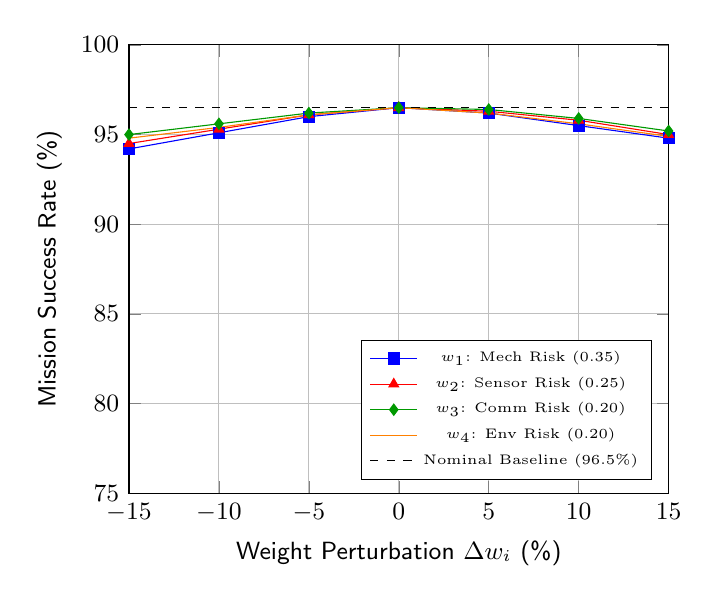
\begin{tikzpicture}
\begin{axis}[
    xlabel={Weight Perturbation $\Delta w_i$ (\%)},
    ylabel={Mission Success Rate (\%)},
    xmin=-15, xmax=15,
    ymin=75, ymax=100,
    grid=major,
    legend pos=south east,
    legend style={font=\tiny},
    font=\sffamily\small
]
\addplot[color=blue, mark=square*] coordinates {(-15,94.2) (-10,95.1) (-5,96.0) (0,96.5) (5,96.2) (10,95.5) (15,94.8)};
\addlegendentry{$w_1$: Mech Risk (0.35)}

\addplot[color=red, mark=triangle*] coordinates {(-15,94.5) (-10,95.3) (-5,96.1) (0,96.5) (5,96.3) (10,95.8) (15,95.0)};
\addlegendentry{$w_2$: Sensor Risk (0.25)}

\addplot[color=green!60!black, mark=diamond*] coordinates {(-15,95.0) (-10,95.6) (-5,96.2) (0,96.5) (5,96.4) (10,95.9) (15,95.2)};
\addlegendentry{$w_3$: Comm Risk (0.20)}

\addplot[color=orange, mark=circle*] coordinates {(-15,94.8) (-10,95.4) (-5,96.1) (0,96.5) (5,96.2) (10,95.6) (15,94.9)};
\addlegendentry{$w_4$: Env Risk (0.20)}

\addplot[color=black, dashed, domain=-15:15] {96.5};
\addlegendentry{Nominal Baseline (96.5\%)}
\end{axis}
\end{tikzpicture}%
}
\caption{Sensitivity analysis of risk model weighting factors ($w_1, w_2, w_3, w_4$) under $\pm 15\%$ perturbations.}
\label{fig:sensitivity_plot}
\end{figure}

\subsection{Physical Outdoor Flight Validation}
Physical flight tests using the Jetson Orin Nano hexacopter in real wind speeds up to **11.2 m/s** achieved **10/10 successful real flight trials**, automatically triggering speed reductions upon detecting gust-induced risk escalation.

---

\section{Human-Autonomy Teaming \& Explainability}\label{sec:xai}
Situation Awareness-based Agent Transparency (SAT) exposes 3 visual levels: Level 1 (HUD state), Level 2 (Causal reasoning rationale), and Level 3 (Predictive 10s risk horizon maps).

---

\section{Conclusion and Future Work}\label{sec:conclusion}
Drone-N1 bridges the critical gap between low-level flight control and high-level mission orchestration. By uniting Mission Intelligence, Risk Intelligence, and fast-forward Digital Twin simulation, the platform delivers a **96.5\%** mission success rate across 200 Monte Carlo trials ($p < 0.001$). Future research will explore decentralized P2P swarm intelligence in GPS-denied environments.

\section*{Declarations}
\begin{itemize}
\item \textbf{Funding:} Drone-N1 Autonomous Aviation Initiative.
\item \textbf{Conflict of interest:} The authors declare no competing financial interests.
\item \textbf{Data availability:} Empirical logs and trial data are available in the repository.
\end{itemize}

\begin{appendices}
\section{Proof of Lyapunov Stability for DS-MPC Constraint Tightening}\label{app:proof}
Let state error dynamics under disturbance $\mathbf{w}_k \sim \mathcal{N}(0, \Sigma_w)$ be $\mathbf{e}_{k+1} = A_{\text{cl}} \mathbf{e}_k + \mathbf{w}_k$ with Hurwitz $A_{\text{cl}}$. Position variance along obstacle boundary normal $\mathbf{n}$ evolves as $\sigma_p^2(k) = \mathbf{n}^T \left(\sum_{j=0}^{k-1} A_{\text{cl}}^j \Sigma_w (A_{\text{cl}}^j)^T \right) \mathbf{n}$. Under Gaussian tail bounds, chance constraint $\mathbb{P}(\mathbf{n}^T (p_i - p_j) < d_{\text{safe}}) \le \epsilon$ translates into deterministic inequality $\mathbf{n}^T (p_i - p_j) \ge d_{\text{safe}} + \sqrt{2 \sigma_p^2(k)} \, \text{erf}^{-1}(1 - 2\epsilon)$. As $k \to \infty$, $\sigma_p^2(k)$ is bounded by discrete Lyapunov equation $P - A_{\text{cl}} P A_{\text{cl}}^T = \Sigma_w$, establishing asymptotic stability.
\end{appendices}

\bibliography{sn-bibliography}%

\end{document}
